\documentclass{standalone}
\usepackage{tikz}
\usepackage{verbatim}
\begin{document}
\pagestyle{empty}
  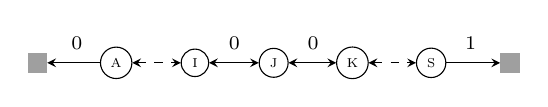
\begin{tikzpicture}
    \node[draw,rectangle,fill,gray!75] (l) at (-3, 0) {};
    \node[draw,circle,scale=2/3] (a) at (-2, 0) {\scriptsize A};
    \node[draw,circle,scale=2/3] (b) at (-1, 0) {\scriptsize I};
    \node[draw,circle,scale=2/3] (c) at (+0, 0) {\scriptsize J};
    \node[draw,circle,scale=2/3] (d) at (+1, 0) {\scriptsize K};
    \node[draw,circle,scale=2/3] (e) at (+2, 0) {\scriptsize S};
    \node[draw,rectangle,fill,gray!75] (r) at (+3, 0) {};
    \draw[-stealth]  (a) -- (l);
    \draw[stealth-stealth, dashed] (a) -- (b);
    \draw[stealth-stealth] (b) -- (c);
    \draw[stealth-stealth] (c) -- (d);
    \draw[stealth-stealth, dashed] (d) -- (e);
    \draw[-stealth]  (e) -- (r);
    \foreach \x in {-0.5, ..., 0.5} {
      \node at (\x, 0.25) {\scriptsize 0};
    }
    \node at (2.5, 0.25) {\scriptsize 1};
    \node at (-2.5, 0.25) {\scriptsize 0};
  \end{tikzpicture}
\end{document}